The given curve 
\begin{align}
	y =\frac{1}{x-1}
\end{align}
can be expressed as 
\begin{align}
	xy - y - 1 = 0 \label{eq:solutions/1/14/eq:hyperbola}
\end{align}
Hence, we have
\begin{align}
	\vec{V} = \frac{1}{2}\myvec{0 & 1 \\ 1 & 0}, 
	\vec{u} = \frac{1}{2}\myvec{0 \\-1},
	f = -1
\end{align}
Since $\mydet{\vec{V}} < 0$, the equation \eqref{eq:solutions/1/14/eq:hyperbola} represents hyperbola.
To find the values of $\lambda_1$ and $\lambda_2$, consider the characteristic equation,
\begin{align}
	\mydet{\lambda\vec{I} - \vec{V}} &= 0\\
	\implies \mydet{\myvec{\lambda & 0\\0 & \lambda} - \myvec{0 & \frac{1}{2} \\ \frac{1}{2} & 0}} &= 0\\
	\implies \mydet{ \lambda & \frac{-1}{2} \\ \frac{-1}{2} & \lambda} &= 0\\
	\implies \lambda_1 &= \frac{1}{2} , \lambda_2 = \frac{-1}{2}
\end{align}
In addition, given the slope -1, the direction and normal vectors are given by 
\begin{align}
	\vec{m} = \myvec{1 \\ -1} \\
	\vec{n} = \myvec{ 1 \\ 1}
\end{align}
The parameters of hyperbola are as follows:
\begin{align}
	\vec{c} &= -\vec{V}^{-1}\vec{u} \\
	&= -\myvec{0 & 2\\ 2 & 0}\myvec{0 \\ -\frac{1}{2}} \\
	&= \myvec{1 \\ 0}\\
	axes &= \begin{cases}
	\sqrt{\frac{\vec{u}^T\vec{V}^{-1}\vec{u} - f}{\lambda_1}} = \sqrt{2}\\
 \sqrt{\frac{f-\vec{u}^T\vec{V}^{-1}\vec{u}}{\lambda_2}} = \sqrt{2}
\end{cases}
\end{align}
which represents the standard hyperbola equation,
\begin{align}
	\frac{x^2}{2} - \frac{x^2}{2} = 1
\end{align}
The points of contact are given by 
\begin{align}
  \tiny{K} &=\pm \sqrt{\frac{\vec{u}^T\vec{V}^{-1}\vec{u} - f}{\vec{n}^T\vec{V}^{-1}\vec{n}}}
  = \pm \frac{1}{2}\\
  \vec{q} &= \vec{V}^{-1}(k\vec{n}-\vec{u})\\
  \vec{q_1} &= \myvec{0 & 2\\2 & 0} \sbrak{\frac{1}{2}\myvec{1 \\ 1} - \myvec{0\\ \frac{-1}{2}}}\\
  &= \myvec{2 \\ 1}\\
  \vec{q_2} &= \myvec{0 & 2\\2 & 0} \sbrak{\frac{-1}{2}\myvec{1 \\ 1} - \myvec{0\\ \frac{-1}{2}}}\\
  &= \myvec{0 \\ -1}
\end{align} 
$\therefore$ The tangents are given by
\begin{align}
	\myvec{1 & 1} \brak{\vec{x} - \myvec{2 \\ 1}} = 0 \\
	\myvec{1 & 1} \brak{\vec{x} - \myvec{0 \\ -1}} = 0
\end{align}
The desired equations of all lines having slope -1 that are tangents to the curve $\frac{1}{x-1}, x \neq 1$ are given by
\begin{align}
	\myvec{1 & 1}\vec{x} &= 3 \\
	\myvec{1 & 1}\vec{x} &= -1 
\end{align}
The above results are verified in the following figure.
\begin{figure}[h!] \label{eq:solutions/1/14/fig:tangents}
	\centering
	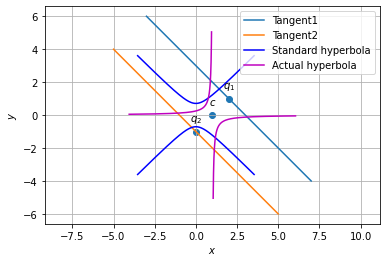
\includegraphics[width=\columnwidth]{./solutions/1/14/graph7.png}
	\caption{The standard and actual hyperbola.}
\end{figure}
